%%%%%%%%%%%%%%%%%%%%%%%%%%%%%%%%%%%%%%%%%%%%%%%%%%%%%%%%%%%%%%%%%%%%%%%%
\chapter{Background and Motivation}
%%%%%%%%%%%%%%%%%%%%%%%%%%%%%%%%%%%%%%%%%%%%%%%%%%%%%%%%%%%%%%%%%%%%%%%%

%%%%%%%%%%%%%%%%%%%%%%%%%%%%%%%%%%%%%%%%%%%%%%%%%%%%%%%%%%%%%%%%%%%%%%%%
\section{Graph Neural Networks}
%%%%%%%%%%%%%%%%%%%%%%%%%%%%%%%%%%%%%%%%%%%%%%%%%%%%%%%%%%%%%%%%%%%%%%%
Given a graph containing nodes, edges, and features, Graph Neural Networks (GNNs) output a per-node \textit{embedding} for each node in the graph.
An embedding is a $d$-dimensional representation of aggregated feature information from a node's neighborhood. 
Similarity in the embedding space has different meaning based on the learning task, such as similarity of node type (a node classification task) \cite{GCN_2016} or likelihood of edge existence (a link prediction task) \cite{LinkPredictionGNN_2018}. 

% In this work we will consider the case where graphs are homogeneous (one node type) and only nodes have associated features.

Borrowing notation from P3 \cite{P3_2021}, we can generally represent the embedding for a node $v$ at layer $k$ as $h_v^k$, where
\begin{align} \label{GNN Equation}
    h_v^k = \sigma \biggl(
         W^k \cdot 
         \mathtt{COMBINE}^{(k)} \left(
            h_v^{k-1},
            \mathtt{AGG}^{(k)} \left( 
                    \{ h_u^{k-1} \mid u \in N(v) \}
                \right) 
         \right)
     \biggl)
\end{align}
\begin{align*}
    \sigma &= \text{Nonlinear function} \\
    W^k &= \text{Trainable weight matrix for layer $k$} \\
    N(v) &= \text{Neighborhood of node v}
\end{align*}
$\mathtt{AGG}^{(k)}$ is a function that aggregates the previous layer embeddings of node $v$'s neighborhood. 
$\mathtt{COMBINE}^{(k)}$ is a function that combines that the result of $\mathtt{AGG}^{(k)}$ with the $v$'s own last layer embedding. 
The first layer embedding for node $v$, $h_k^0$, is just its original features.

The choice of $\mathtt{AGG}^{(k)}$ and $\mathtt{COMBINE}^{(k)}$ are depend on specific GNN architecture. Graph Convolutional Networks (GCN) \cite{GCN_2016}, GraphSAGE \cite{GraphSAGE_2017}, and Graph Attention Networks (GAT) \cite{GAT_2018} perform different types of aggregations and operations on features, but share the same general aggregation principle.

Since for each layer there is a different $W^k$, GNNs are comprised of $k$ neural networks. Furthermore, each layer requires recursive computation on a node's neighbors. Thus a \textit{$k$-hop neighborhood} must be constructed to run a $k$-layer GNN.
Generally GNNs use 1-5 layers, with 2 layers being a de facto standard \cite{Survey_First_2022}. However, some architectures can use significantly more layers, such as the current SOTA EnGCN model comprising 8 layers \cite{EnGCN_2023}.
Figure \ref{Background: GNN Execution Example} illustrates the construction of a \textit{computation graph} for a $2$-layer GNN. A computation graph describes how necessary nodes and edges participate in GNN computation.


\begin{figure}[h!]
    \begin{minipage}[c]{0.5\textwidth}
        \centering
        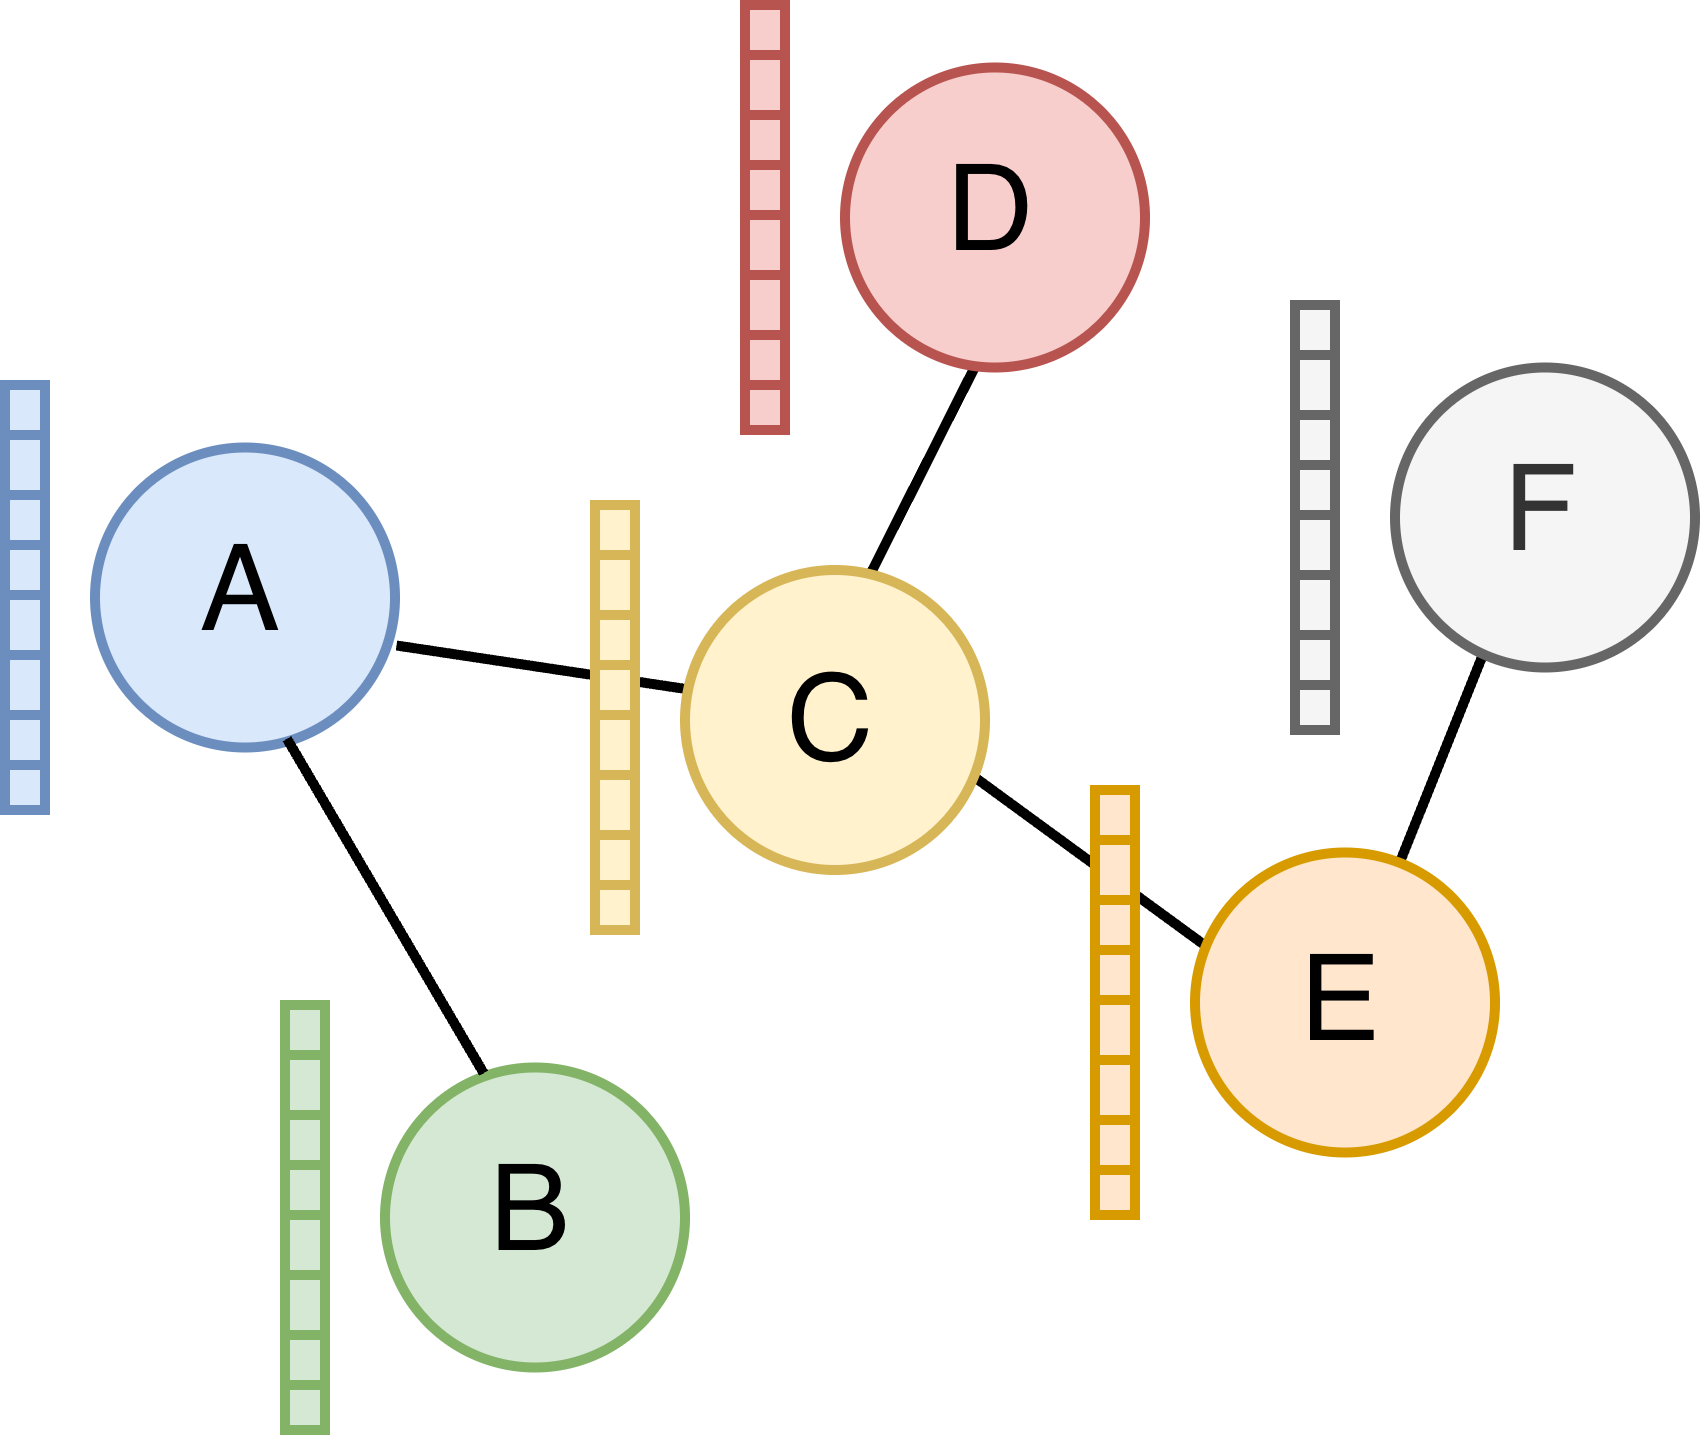
\includegraphics[width=0.85\textwidth]{diagrams/group_meeting_gnn-Graph structure.png}    
        % \caption{Graph structure and associated node features (colored bars).}
    \end{minipage}
    \hfill
    \begin{minipage}[c]{0.45\textwidth}
        \centering
        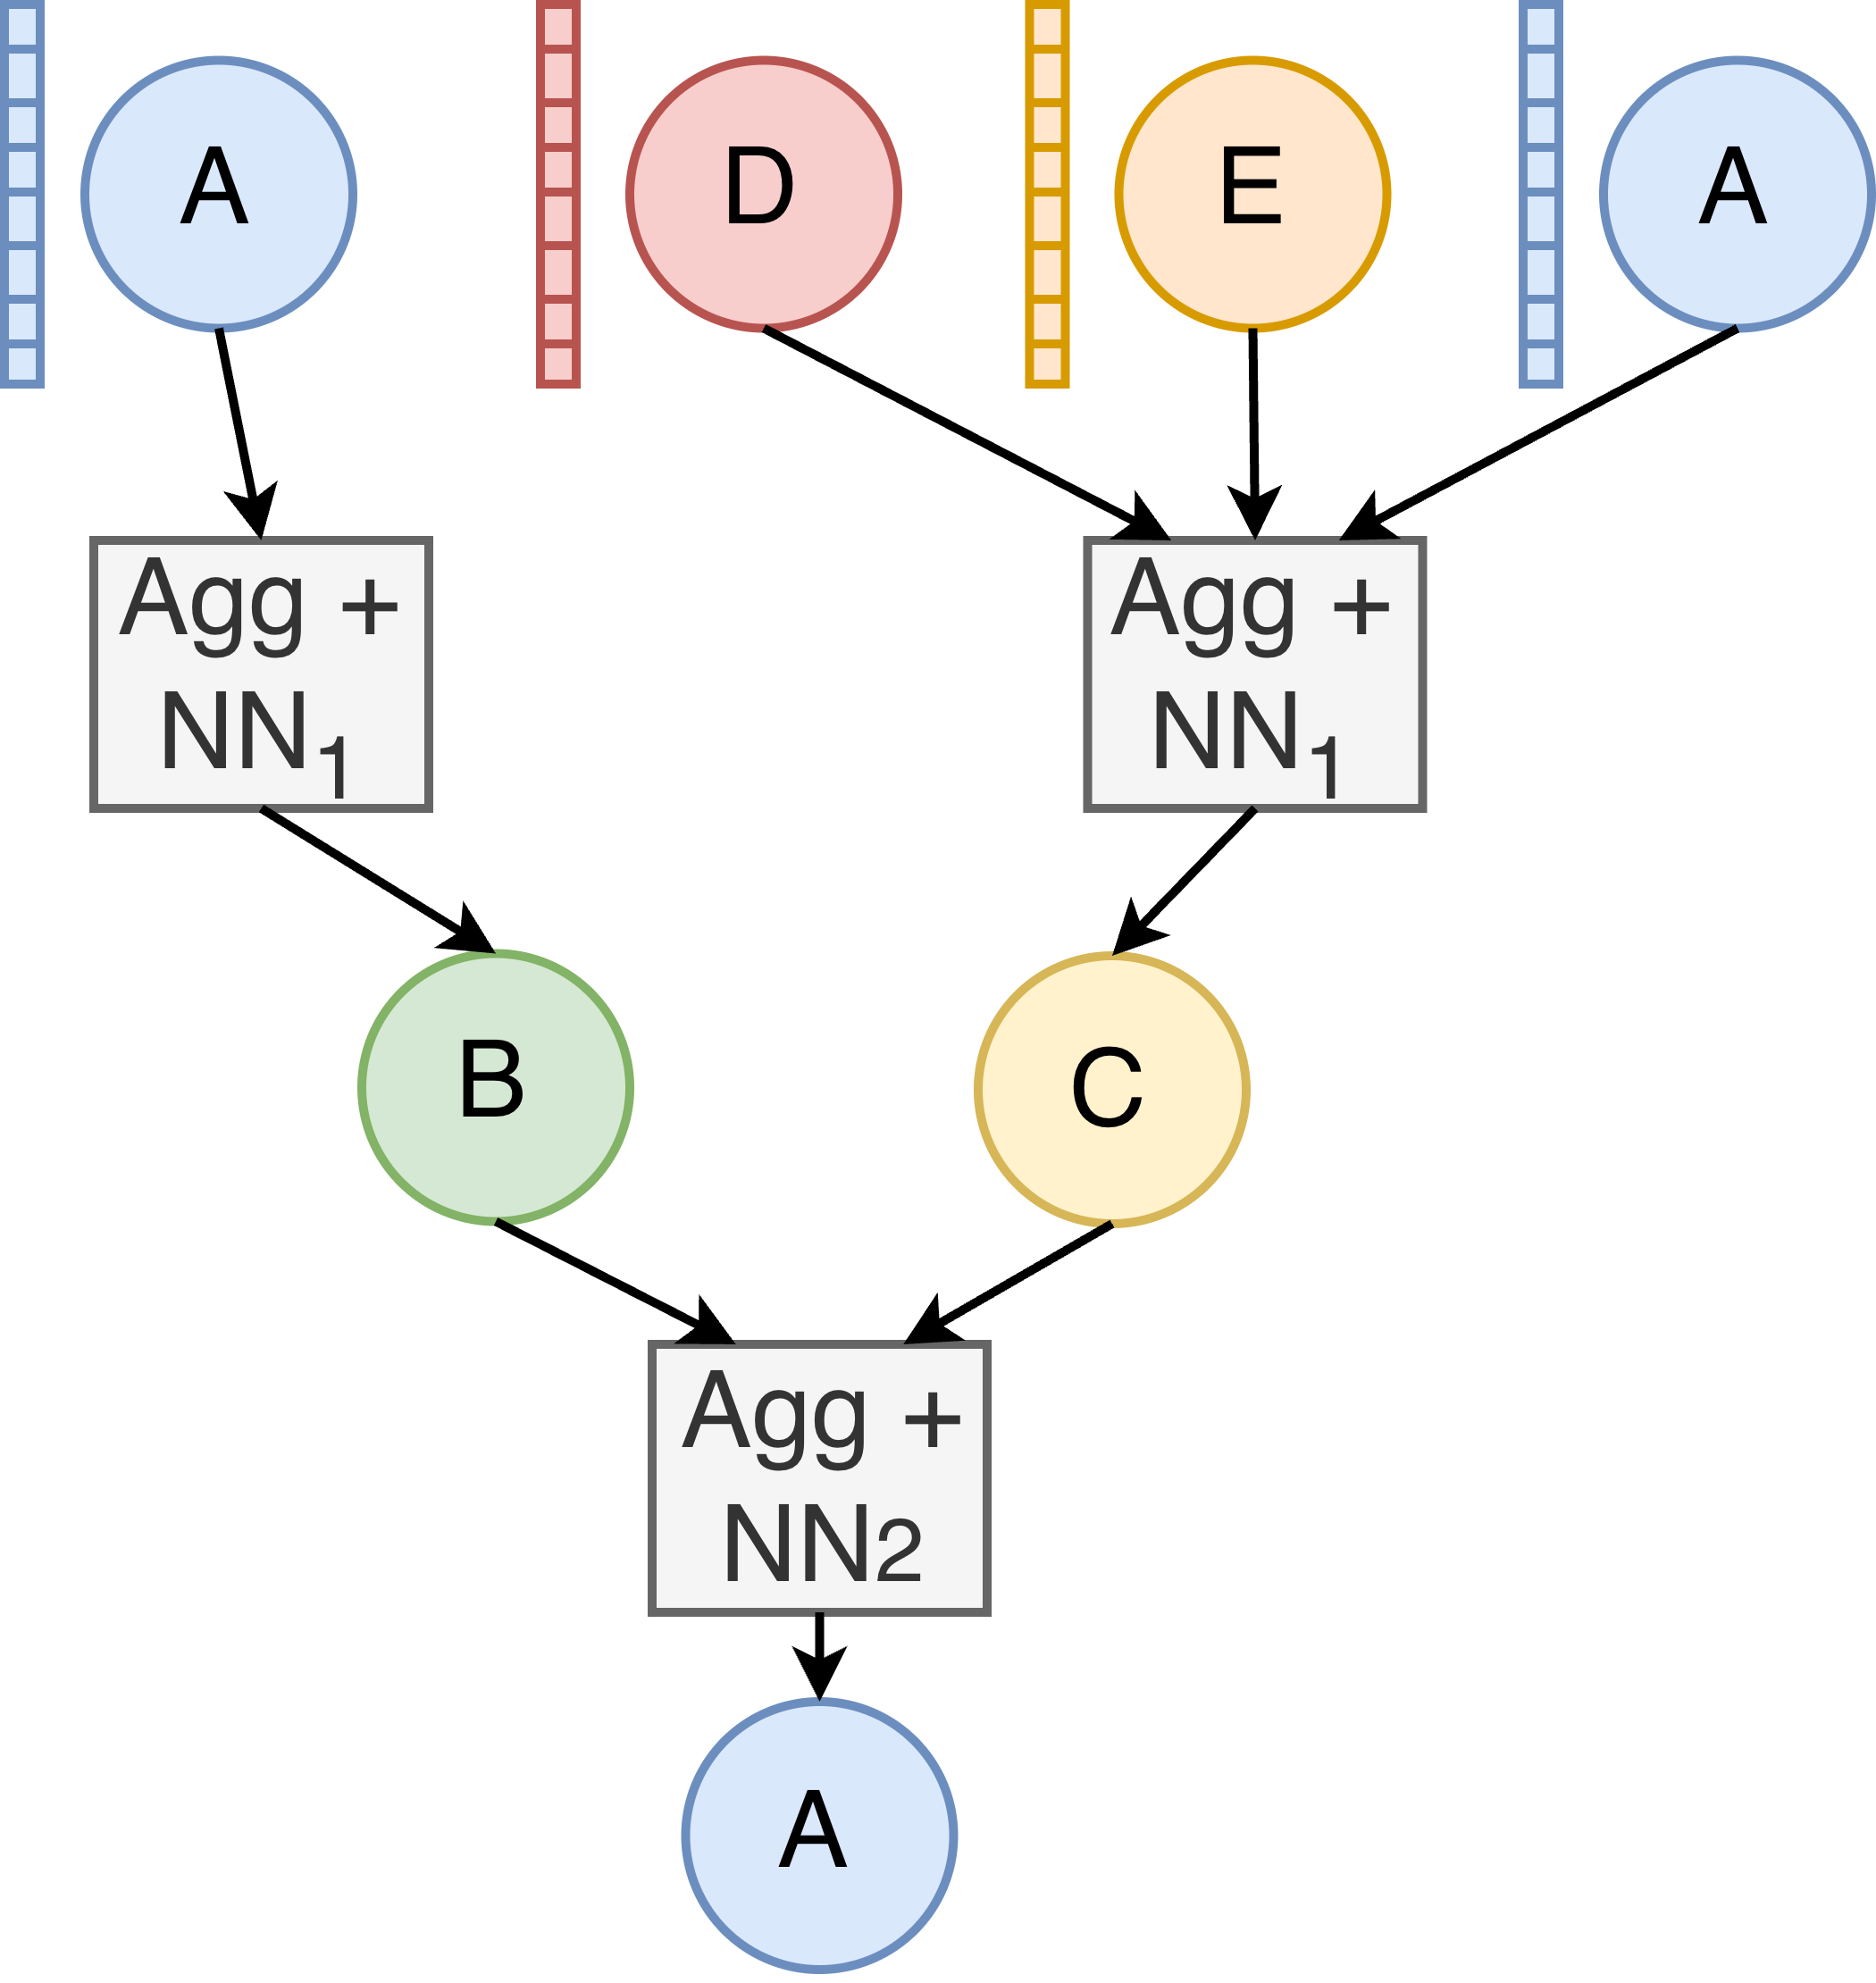
\includegraphics[width=0.95\textwidth]{diagrams/group_meeting_gnn-GNN Execution.png}
        % \caption{2-hop neighborhood and computation graph for node $A$, ignoring self loops.}
    \end{minipage}
    \caption{Graph and associated computation graph for node $A$.}
    \label{Background: GNN Execution Example}
\end{figure}    

%%%%%%%%%%%%%%%%%%%%%%%%%%%%%%%%%%%%%%%%%%%%%%%%%%%%%%%%%%%%%%%%%%%%%%%%
\section{Online GNN Inference}
%%%%%%%%%%%%%%%%%%%%%%%%%%%%%%%%%%%%%%%%%%%%%%%%%%%%%%%%%%%%%%%%%%%%%%%%
% [todo define what inference is?]
Traditionally, GNN inference has been viewed as an \textit{offline} problem, where inference is performed on all nodes in the graph (full graph inference).
Full graph inference is typically used for evaluating trained models or computing node embeddings for future lookup. 
For example, PinSage \cite{Recsys_PinSAGE_2018} first uses MapReduce \cite{MapReduce_2004} to perform full graph inference before storing all node embeddings in a database.
Then, PinSage uses $K$-nearest neighbors to compute embeddings for new queries, enabling it to serve online recommendation requests.
However, this approach, along with other nearest neighbor approaches, suffers from a loss in accuracy compared to directly using a GNN to compute the new embedding.

Therefore, in this work we will view GNN inference as a \textit{online} problem, where a GNN is given a request to compute an embedding for a node or batch of nodes. In this setting, requests consist of nodes, their features, and edges connecting them into the existing graph.

In this section we motivate this online inference formulation and present a concrete taxonomy of the stages of GNN inference.

\subsection{Online Inference Applications}
Online inference has many applications depending on domain.
For example, in a social network graph, an inference request can correspond to computing the embedding for a new user or recomputing embeddings as a result of a new friendship. 
Furthermore, there is no strict requirement that a node is truly "new", meaning that an inference request could correspond to an update of node features.
For example, in a traffic forecasting application, an inference request can be an update of node features that represent a change in traffic conditions.

% Facebook's social network graph in 2013 experienced roughly 86 thousand node or edge updates per second \cite{Graph_Survey_2020}. [todo put this in context]

\subsection{GNN Inference Stages}
While online GNN inference is generally understudied, it shares many similarities with GNN mini-batch training (discussed in Section \ref{Background: Relation to training}). Thus when understanding the steps required to perform GNN inference, we use established taxonomy from mini-batch training work \cite{PaGraph_2020}\cite{GNNLab_2022}\cite{P3_2021}. We break down the stages of GNN inference as follows:

\begin{figure}[h!!!]
    \centering
    \begin{enumerate}
        \item \textbf{Sampling:} Construct $k$-hop neighborhood for target nodes and build logical computation graph describing GNN computation.
        \item \textbf{Data Loading:} Moving necessary data to GPU, comprising two steps.
        \begin{enumerate}
            \item \textbf{Feature gather:} Gather node features corresponding to $k$-hop neighborhood in contiguous CPU buffer.
            \item \textbf{CPU-GPU copy:} Copy buffer with node features and computation graph to GPU.
        \end{enumerate}
        \item \textbf{Model execution:} Perform GNN computation on GPU.
    \end{enumerate}
    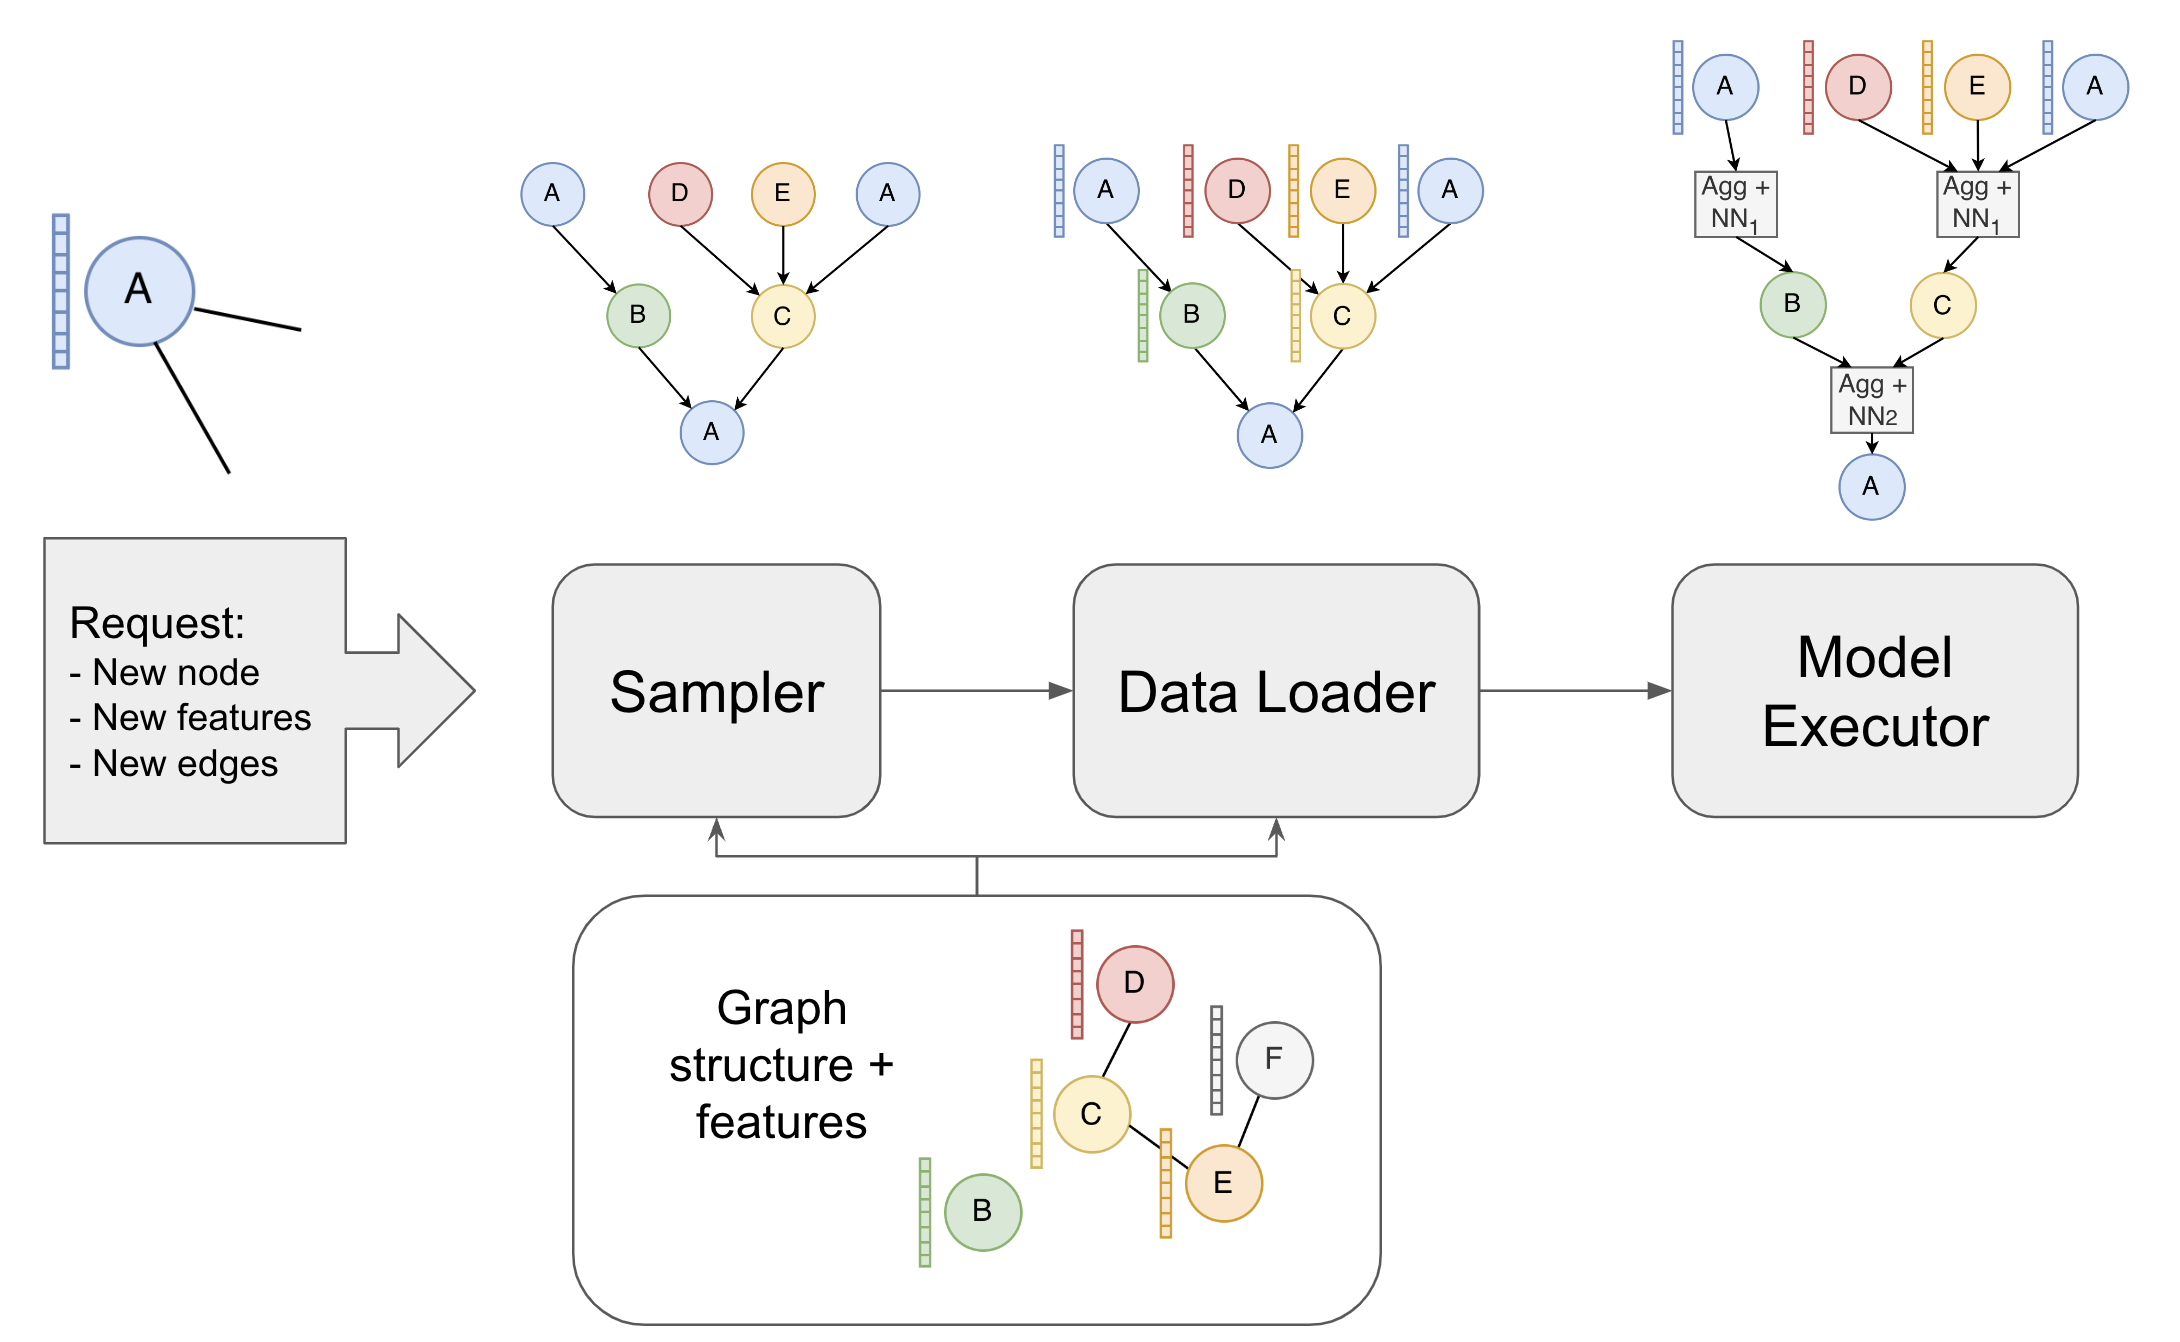
\includegraphics[width=\textwidth]{figures/Compute example.png}
    
    \caption{Online GNN Inference}
    \label{Compute Visualization}
\end{figure}    


%%%%%%%%%%%%%%%%%%%%%%%%%%%%%%%%%%%%%%%%%%%%%%%%%%%%%%%%%%%%%%%%%%%%%%%%
\section{Inference vs. Training} \label{Background: Relation to training}
%%%%%%%%%%%%%%%%%%%%%%%%%%%%%%%%%%%%%%%%%%%%%%%%%%%%%%%%%%%%%%%%%%%%%%%%
In this section we analyze similarities and differences between the inference and training tasks and examine the effectiveness of relevant GNN training optimizations at inference time.

Mini-batch training is a popular technique for GNN training on large graphs where embeddings are only computed for a random subset of the graph per epoch \cite{BGL_2023}. 
This is as opposed to full graph training, where node embeddings and gradients are computed for the entire graph at once, similar to full graph inference.
Mini-batch training is analogous to online inference, and, aside from the high-level goal, the difference is that no backpropagation is needed for inference. We briefly look at prior optimizations for the sampling and data loading stages, with particular emphasis on the latter.

\subsubsection{Sampling Optimizations}
The \textit{neighborhood explosion} problem is a well known issue in the sampling stage.
Since the size of $k$-hop neighborhoods are inherently exponential, constructing these neighborhood and corresponding computation graphs can be expensive. \textit{Neighborhood sampling} helps alleviate this problem by randomly selecting a fixed number or percentage of node neighbors during the sampling stage \cite{GraphSAGE_2017}. 
However, since this can produce a drop in model accuracy, works such as NextDoor \cite{NextDoor_2021} have proposed performing sampling on GPU rather than CPU, yielding significant speedups.
In our system we will leverage this GPU sampling approach.

\subsubsection{Data Loading Optimizations}

Prior GNN training works have observed that data loading can also be a significant bottleneck.
Bus bandwidth between host memory and GPUs can easily be saturated by GNN dataloading. 
For reference, PCIe 3.0 16x and PCIe 4.0 16x unidirectional bandwidth is 16 GB/s and 32 GB/s respectively [todo cite].
Meanwhile, given exponential neighborhood sizes and large feature dimensions, it is easy for transfers of several hundred megabytes to be required for each minibatch.
Therefore, gathering these features in CPU memory and copying them to the GPU can bottleneck training pipelines.

Since GNN models have relatively few parameters compared to traditional DNNs, GPU compute and memory can actually be underutilized during training. Thus several works have proposed caching node features in GPU memory so they no longer need to be copied over from host memory. We are particularly interested in these following GNN training systems implementing feature caches, since we find that data loading is a several bottleneck during inference.

\begin{description}
    \item[PaGraph \cite{PaGraph_2020}] introduces \textit{static feature caching}, proposing a policy where the features of the highest degree nodes in the graph are stored on the GPU prior to training. This cache is \textit{static} since these features features remain permanently in GPU memory until training concludes. A static cache can be used for inference and is low overhead, but has worse cache hit rates than dynamic caches.
    \item[GNNLab \cite{GNNLab_2022}] extends static caching to include a pre-sampling phase, where warmup epochs are run to determine what nodes are most often used and thus should be stored in the cache. Although the pre-sampling approach cannot be directly applied to inference, we build upon the idea of using frequency as a feature for determining cache residents in Section \ref{Design: Policy}.
    \item[BGL \cite{BGL_2023}] uses a dynamic FIFO cache and iterates over the graph in a roughly-BFS manner to exploit the FIFO cache. BGL's approach is reliant on controlling the node order during training time and thus cannot be applied to inference. However, BGL does introduce using NVLinks between GPUs to share cache resources, which we improve upon by enabling greater concurrency in Sections \ref{Design: Multi-GPU} and \ref{Design: Lock-free}.
\end{description}

\subsection{GNN Inference Challenges}
We observe that after adopting the GPU sampling and static caching techniques from GNN training systems, inference latency is still dominated by data loading operations. Figure \ref{GPU Sampling Latency Breakdown} illustrates these results. 

\begin{figure}[h!]
    \centering
    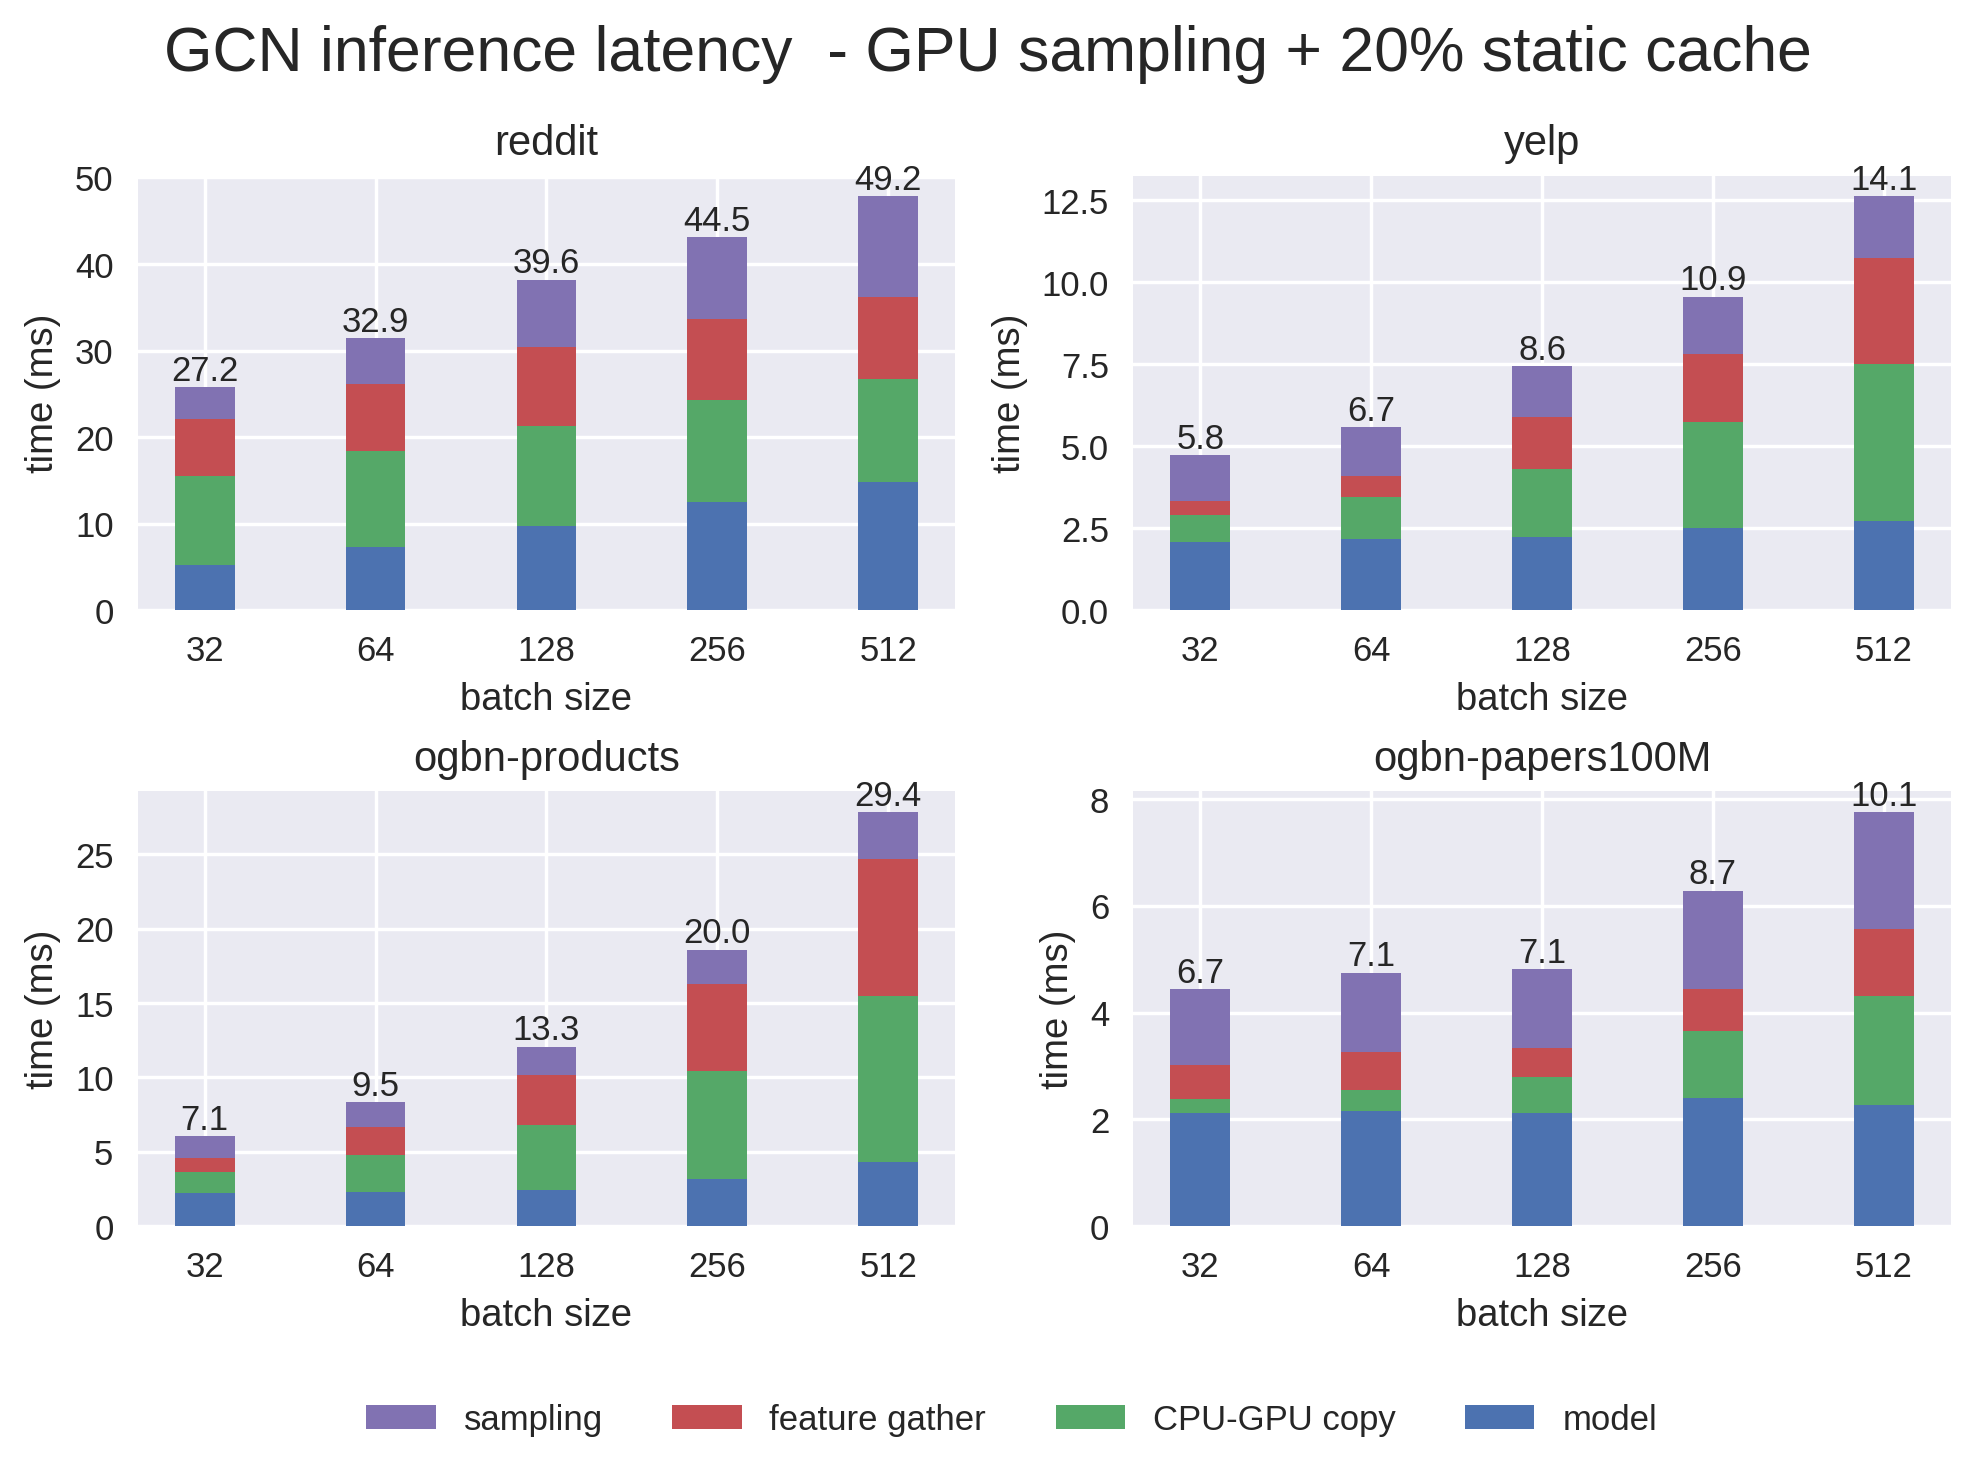
\includegraphics[width=0.8\textwidth]{figures/GCN_latency_breakdown_gpu_sampled_with_cache.png}
    
    \caption{Inference latencies for different graph datasets and request batch sizes (number of target nodes in request). Requests are served by a system using GPU sampling and a static cache large enough to hold 20\% of each graph dataset's node features. The test platform is detailed in Section \ref{Eval: Test hardware}}
    \label{GPU Sampling Latency Breakdown}
\end{figure}    


GNN inference has unique challenges that make it critical to carefully apply optimizations. In particular,

\begin{enumerate}
    \item \textbf{Latency is a key metric at inference time}. During GNN training, throughput is far more important than latency. For example, many training systems try to hide data loading overheads by pipelining additional compute during data transfers. However, pipelining cannot hide latency. As a result, an efficient inference system must directly reduce data loading overhead.
    \item \textbf{Model computation is much faster during inference}. At inference time there is no need to perform backpropagation, meaning that sampling and data loading comprise a larger percentage of inference latency. Furthermore, modern deep learning frameworks such as PyTorch \cite{PyTorch_2019} and TensorFlow \cite{tensorflow2015-whitepaper} offer optimizations that can be enabled at inference time, such as not tracking gradients, which skews this proportion further.
\end{enumerate}


% Reasons why we optimize data lodaing stage
% \begin{enumerate}
%     \item \textbf{Data loading comprises significant portion inference latency}
%     \item \item \textbf{Data loading latency cannot be hidden with pipelining}
%     \item \textbf{Data loading overhead scales with feature dimension}
% \end{enumerate}


